% !TEX root = ../main.tex
\section{Horned Kin} \label{kin::gat}
\DndDropCapLine{W}{hen you contract a horned one, be}
\textit{sure to pay them double.
Fulfill all their needs as they seclude into their workshop, and pay no mind to their uncanny silence.
Most of all, be sure to avoid interrupting them.
Just wait.
The prize that will arrive after they're done working is sure to outshine all your other possessions, and hold a special place in your collection for you and your descendants.}

\hspace*{\fill} --- Orr, Vesjen's master smith.

Citadels carved into the highest of cliff faces.
Mines hidden inside the deepest of ravines.
Workshops rumbling with the sound of hard labor until the darkest of hours.
These are the traits that define the gat.

The gat, marheth'llal rlue, or horned kin are the oldest among the sentient races created by the ets.
Molded as diggers and laborers, their passion for work is ingrained into their very blood.
To date they are known as master miners, builders, and artisans.

Being the first of the kins, they are established and well-developed.
Gats are the builders of the Seven Kingdoms of the Coast, the oldest active nations in Yuadrem.

\subsection*{Beard and Horns}
    The horned kin was designed in the image of goats, and share their horns, facial features, and digitigrade feet.
    They stand in a hunched manner and are generally slender.
    Gats are covered by a thick layer of fur ranging in hues from light blonde to absolute black.
    Many enjoy growing a beard.

    Gats' eyes are of strong colors, usually light blue, yellow, orange, or light brown.
    Like goats, their pupils are rectangular and elongated.
    The manner in which each gat's beard and horns grow is unique, and most take pride in these features, showing them off whenever possible.

    Gats are genderless creatures.
    All gats are born with a pair of seeds hidden in a small sack between their legs.
    Around the age of 30, a gat reaches physical maturity.
    This is signalled by a slight swelling in these seeds, which they can now cut and plant under a thick layer of rich soil.

    While underground, the seed will grow by leeching nutrients off the earth.
    After a gestation period of around 2 years, the gat will dig their way up from the ground and emerge as a somewhat competent infant.
    A gat would-be-parent must always be careful about where to plant their seed, for if a newborn sees the sun or any strong light during their first days, they run the risk of being permanently blinded.

\subsection*{Adaptable and Hardy}
    Gat share many traits with the common goat.
    They dwell on bleak mountaintops, deep ravines, rocky hills, and open plains.
    While adult gats are not sensitive to sunlight, most prefer dark places.
    These predilections lead to gat towns and cities being built underground or in harsh cliff faces.

    Never satisfied with their homes, the horned kin's hubris leads to their cities to reach depth and size.
    Raids against smaller gat city-state are common, and the gats take them as a chance to test their impenetrable defenses, complex traps, and combat-hardened military skills.

\subsection*{Peaceful Demeanor}
    The horned kin are peaceful creatures and mostly shun external conflict.
    They are very sociable creatures, and all city-states have one large marketplace in their center for merchants and caravans to settle in.
    Surrounded by inns and taverns, these markets act as the commerce hubs of the city.

    Community lifestyle is very important to gats, and most wouldn't flinch to give their lives for their city-state.
    Due to the gats' slow reproductive cycle, their cities are very welcoming to other species.
    It's common to find cities and towns where less than half of the total population is gat.
    They treat other species as kin, but high political and military ranks are exclusive to gats.

\subsection*{Impulse towards Greatness}
    It is rare for a gat to willingly leave their home, and most spend their entire lives in one city-state.
    However, some do feel the call to adventure, and most follow it to gather rare crafting materials or to fulfill a task needed by their community.

    Gats are meticulous individuals, and this naturally extends to adventurers.
    They won't step into the wilderness unprepared, sparing no expense in armor, weapons, utilities, and the training to use all of this.

    Gats are naturally family-oriented, and its very rare for one gat to abandon their progeny.
    In the rare occasion that a gat does decide to leave their community behind, it is written law to leave one child or seed planted back home.

    This tradition serves a double purpose.
    First, the child acts as a magnet to their parent.
    Second, in the event that the child is orphaned, their mere presence at least maintains a steady population number.
    These gats are the ``Children of the Collective'', and it is tradition that they are taken care of by the whole city, thus nurturing a strong sense of community.

\subsection*{Gat Names}
    All gat tongues are simple and practical languages, and the horned ones have a tendency towards easy to pronounce names.
    A parent gives their child their name once they gain independence, and its rare for a gat to change it.
    Gats don't use family names, preferring instead to wear their main profession as a surname.

    \paragraph{Names}
    Adrevik, Ani, Anush, Armen, Avag, Gagik, Garen, Gevog, Gohar, Grigor, Hak, Harig, Hovsep, Jirar, Kevon, Khadzak, Marim, Narek, Pagran, Poghos, Ruben, Sivadr, Sona, Vahagn, Vefan.

    \paragraph{Surnames}
    Axgat, Bonecarver, Bowyer, Caretaker, Cook, Dyer, Engraver, Farmer, Fishergat, Glassblower, Gemcutter, Guard, Mason, Metalsmith, Miner, Speargat, Trader, Trapper, Weaponsmith, Woodworker.

\subsection*{Traits}
    Your gat character's hardiness and tendency towards craftsmanship gives them the following set of skills:

    \subparagraph{Ability Score Increase} Your Constitution score increases by 2.

    \subparagraph{Age} Gats mature slowly, but they live very long lives.
    You are sexually mature at around 30 years, and live to around 350 years.

    \subparagraph{Alignment} Industrious and strong, gats focus more on getting things done rather than morals or ethics.
    They have a tendency towards fairness and justice, and therefore are inclined towards the indigo tide.

    \subparagraph{Size} Gats typically range from 1.2 to 1.5 meters.
    Your size is medium.
    They aren't too slender or stout for their size, weighing on average 50 kg.

    \subparagraph{Speed} Your base walking speed is 9 meters.

    \subparagraph{Stable Footing} You are not slowed by difficult terrain caused by rocks, gravel, sheer faces, and other such obstacles.

    \subparagraph{Keratin Horns} You know the Push action (See page \pageref{act::push}), using your strong horns to shove your target.

    Additionally, your horns are a melee weapon that deals 1d4 plus your Strength modifier in bludgeoning damage.

    \subparagraph{Craftsgatship} You are competent with a set of artisan's tools of your choice.

    \subparagraph{Strange Mood} Periodically, individual gat are struck with an idea for a masterwork artifact and enter a strange mood.
    Only with a great force of will can a gat ignore this pull, and not even the strongest can fully stop the craving.

    If you are at least 30 years old, roll a d100 whenever you take a long rest.
    % You can choose to roll this twice.
    On a 100, you are struck by a strange mood.
    The materials required for your masterwork item can either be chosen by you or by the DM.
    They must be related to the proficiency given by your Craftsgatship trait and at least one of them must be either hard to find or very expensive.

    At the start of every sucsequent long rest, you must succeed on a Wisdom saving throw of a DC equal to 8 + the number of months since your strange mood started.
    On a fail, the need to work on your craft consumes you.
    If you fail to work on the object in any way during the long rest, your restlessness prevent you from gaining its benefits.

    It takes you a month of work in total to craft the artifact, which can be paused between

    It takes you 2 months of work to craft the artifact, but after you start you can indefinitely pause the production as long as you can properly secure it.
    The masterwork item produced has a value of 100,000 GP, but it's very rare to see a gat willingly part with it.
    These items are usually declared as family heirlooms, personal keepsake, or an offering to a king, leader, or deity.

    Weapons, armor, or similar objects crafted in a strange mood are +2, and are of specially exquisite quality.

    \subparagraph{Languages} You know how to speak, write, and read Avshenese and one additional language of your choice.

    \subparagraph{Feats} From your kin, the feats available to you are
    \textbf{Efficient Craftsgat} (page \pageref{feat::efficientcraftsgat}),
    \textbf{Force of Will} (page \pageref{feat::forceofwill}),
    \textbf{Goat's Strength} (page \pageref{feat::goatsstrength}),
    \textbf{Legendary Craftsgat} (page \pageref{feat::legendarycraftsgat}),
    \textbf{Powerful Build} (page \pageref{feat::powerfulbuild}),
    \textbf{Relentless Endurance} (page \pageref{feat::relentlessendurance}), and
    \textbf{Stonecutting} (page \pageref{feat::stonecutting}).

\begin{figure}[!b]
    \centering
    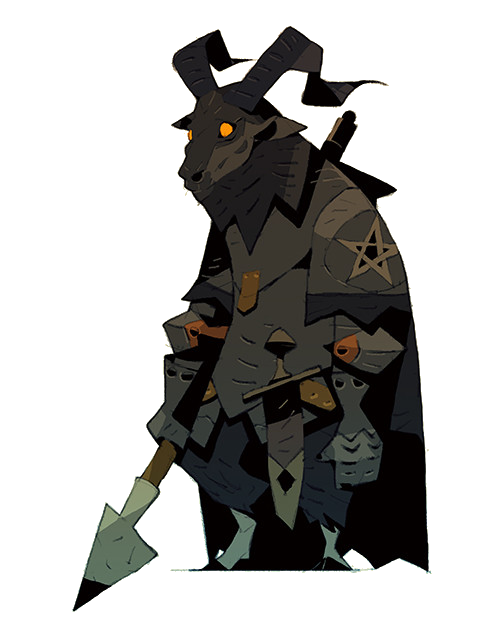
\includegraphics[width=0.47\textwidth]{04kins/img/11gat_knight.png}
\end{figure}

\newpage

\subsubsection{Noves Gat}
    Acclimated to the highest mountains and deepest ravines, cliff gats are the most common of the horned kin.
    Builders of the immense gat city-states, it's very rare to see a cliff gat not actively pursuing their craft.

    \subparagraph{Ability Score Increase} Your time spent in civilization has given you a profound common sense and a general grasp on almost any subject.
    Your Intelligence score is increased by 1.

    \subparagraph{Gat Toughness} Your hit point maximum increases by 1, and it increases by 1 every time you gain a level.

    \subparagraph{Expert Craftsgatship} Noves gats are renowned worldwide for their crafts, and even the untrained eye can recognize an item made by one.
    You are an expert with the artisan's tools associated to your Craftsgatship trait.

    The value of the item you produce in a strange mood is increased to 250,000 GP.
    If you make a weapon, armor, or similar item, it is a +3 item.
    Additionally, you must roll your Strange Mood wisdom saving throw twice at the beginning of every month.

    \subparagraph{Feats} From your subrace, the feats available to you are
    \textbf{Gat Resilience} (page \pageref{feat::gatresilience}),
    \textbf{Mountainborn} (page \pageref{feat::mountainborn}), and
    \textbf{Stone's Endurance} (page \pageref{feat::stonesendurance}).

\subsubsection{Bughna Gat}
    In the year 102 AS, the army of healing invaded Ctereth's dwellings and plundered a great haul of qualar.
    These qualar restored the minds of many gats, who became known as the bughna gats.
    % While their minds were recovered, the habits they learned as lost ones have never truly been abandoned.

    Bughna gats feel constrained in cities, and tend to abandon city-states at a young age, freely exploring the outside world.
    % Despite their nature, gats are never truly free of their sense of community.
    Bughna gats tend to travel in packs comprised by varied kins and ethnic groups.

    \subparagraph{Ability Score Increase} Your balance and ability to walk on the steepest of hills is unmatched, and your Dexterity score is increased by 1.

    \subparagraph{Fleet of Foot} Your base walking speed increases by 3 meters.

    \subparagraph{See Them Coming} You have advantage on initiative rolls while in plains, grasslands, and any other open natural environment.

    \subparagraph{Feats} From your subrace, the feats available to you are
    \textbf{Exercised Mind} (page \pageref{feat::exercisedmind}),
    \textbf{Hardy} (page \pageref{feat::hardy}), and
    \textbf{Mirthful Leaps} (page \pageref{feat::mirthfulleaps}).

\subsubsection{Treb Gat}
    While many of the gat lost ones were recovered, most of those who wandered off to the dead sea could never be found due to the toxic mist.
    Here they became the Treb Gat, and eventually acquired qualar back via unknown means.

    These gats are far removed from their calm origins, having to survive the harsh and hostile environment.
    Treb gats have large and muscular bodies, large horns, and dirty, patchy hair.

    \subparagraph{Ability Score Increase} Your restlessness knows no bounds.
    Your Strength score is increased by 1.

    \subparagraph{Size} Treb gats tend to be much larger than their common brethren, measuring between 160 and 200 cm and weighting between 90 and 120 kg.
    Your size is still medium.

    \subparagraph{Uncanny Brutality} While in combat, you are absorbed by a primal rage.
    You have disadvantage on any attacks made with finesse, martial weapons without the heavy property, and ranged weapons.

    \subparagraph{Hammering Horns} You are never unarmed.
    The damage die of your horns is increased to a d6.

    \subparagraph{Savage Attacks} When you score a critical hit with a melee weapon attack, you can roll one of the weapon's damage die one additional time and add it to the extra damage of the critical hit.

    \subparagraph{Fell Mood} When you are struck by a strange mood, the need to craft an exquisite artifact is replaced by an unrelenting urge to kill.
    You have to choose your prey from either a renowned hero, an ancient being, or a forgotten beast.

    After the deed is done, you can craft a disquieting artifact from the creature's remains, following the normal rules of a strange mood.
    All the other conditions of the trait remain the same, replacing the need to gather materials with the insatiable craving to hunt said creature.

    \subparagraph{Feats} From your subrace, the feats available to you are
    \textbf{Goring Rush} (page \pageref{feat::goringrush}),
    \textbf{Imposing Presence} (page \pageref{feat::imposingpresence}), and
    \textbf{Relentless Striker} (page \pageref{feat::relentlessstriker}).

\begin{figure}[!b]
    \centering
    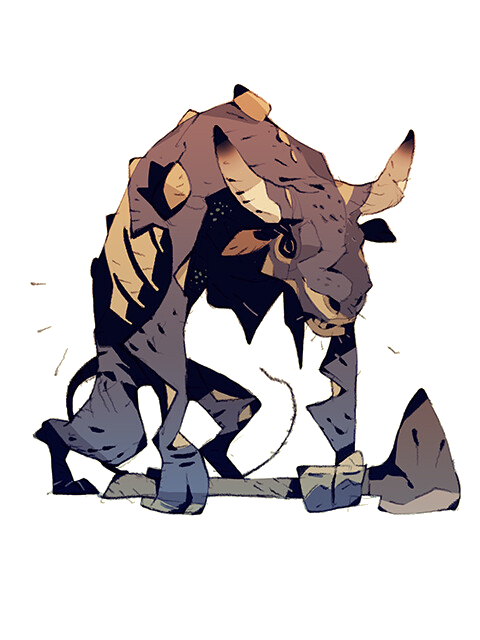
\includegraphics[width=0.48\textwidth]{04kins/img/11gat_treb.png}
\end{figure}

\newpage
